\documentclass[a4paper, 14pt]{article}
\usepackage[dvipsnames]{xcolor}
\usepackage[top=70pt,bottom=70pt,left=48pt,right=46pt]{geometry}
\definecolor{header}{RGB}{92,184,92}
\definecolor{defenition}{RGB}{217,83,79}
\definecolor{main_title}{RGB}{66,139,202}
\definecolor{sub_header}{RGB}{91,192,222}
\usepackage[english, russian]{babel}
\usepackage[utf8]{inputenc}
\usepackage{amsmath}
\usepackage{listings}
\usepackage{graphicx}
\usepackage{amsmath}
\title{\textcolor{main_title}{Исследование фотопроводимости полупроводников}}
\author{Шмаков Владимир Евгеньевич - ФФКЭ гр. Б04-105}






\begin{document}
\maketitle

\section*{\textcolor{header}{Цель работы}}

\begin{enumerate}
    \item Познакомиться с явлением фотопроводимости
    \item Оценить ширину запрещенной зоны CdS и CdSe
\end{enumerate}

\section*{\textcolor{header}{Теоретические сведения}}

	
Электропроводность полупроводника увеличивается под действием света. 
Это явление называется \textcolor{defenition}{\textbf{фотопроводимостью}} или {внутренним фотоэффектом}. 

В отсутствии света в полупроводнике присутствует некоторое количество носителей тока: электроны переходя из валентной зоны в зону проводимости (в случае наличия примесей возможны также переходы с донорных на акцепторные уровни) в результате теплового движения. Количество таких носителей определяется температурой кристалла, они называются равновесными и составляют темновой ток. 

Фотопроводимость проявляется в случае, если энергия квантов превышает некоторое пороговое значение. Для собственной фотопроводимости это значение равно ширине запрещенной зоны, а в случае примесной --- энергии ионизации соответствующего уровня. Минимальная частота света, при которой возможно появление неравновесных электронов (то есть, электронов фотопроводимости), называется красной границей фотоэффекта. При этом можно считать, что включение света не влияет на концентрацию равновесных электронов. 








\section*{\textcolor{header}{Методика}}
\subsection*{\textcolor{sub_header}{Оборудование}}

\begin{itemize}
    \item Призменный монохроматор 
    \item Лампа накаливания 
    \item Неоновая Лампа - для проверки градуировки
    \item Набор линз 
    \item Вольтметр
    \item Исследуемые образцы 
\end{itemize}

\subsection*{\textcolor{sub_header}{Экспериментальная установка}}

В работе исследуются два образца: CdS и CdSe. 
Схема установки приведена на рисунке \ref{pic:scheme}. 
Свет от источника И с помощью линзы Л фокусируется на щель монохроматора УМ-2, 
находящуюся в фокусе линзы Л$_1$. Пучое света разлагается призмой П, и выходная щель, находящаяся в фокусе линзы Л$_2$, вырезает отпределенную область спектра. После прохождения монохроматора свет падает на ячейку Я с образцом. Вольтметр В7-34 нужен для измерения тока через образец. 

\begin{figure}[h]

    \centering	
    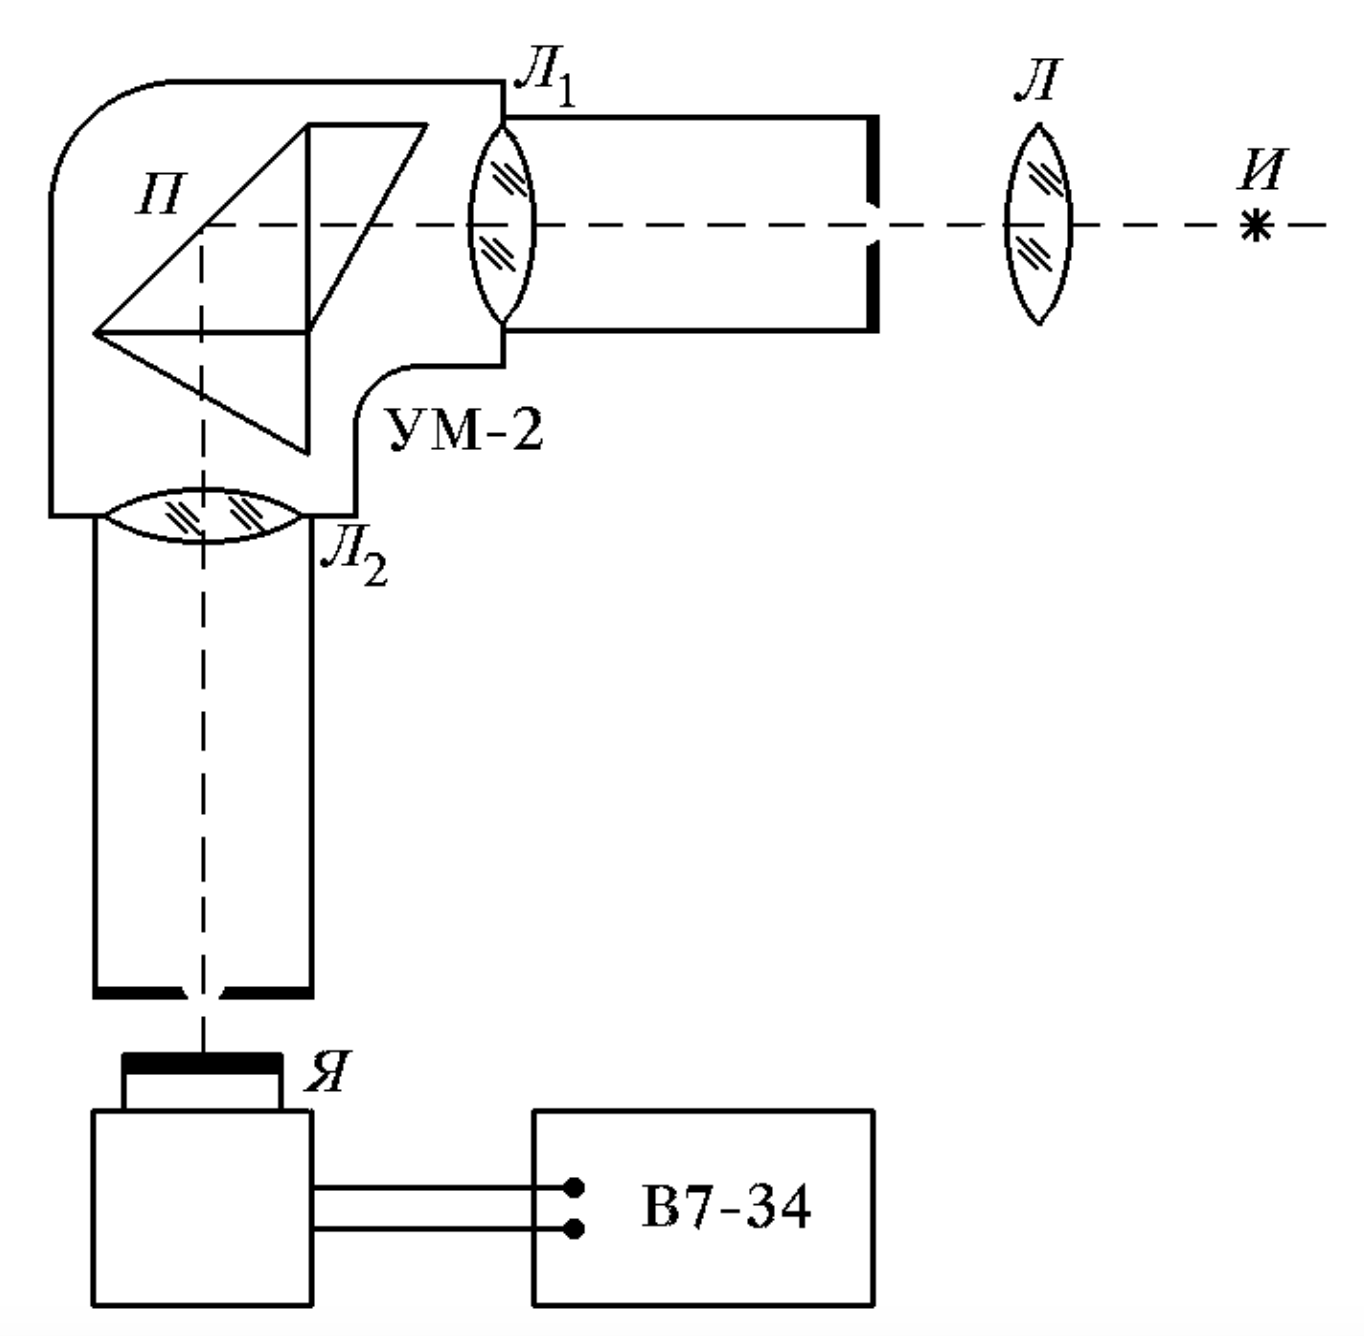
\includegraphics[width=0.4\textwidth]{lab.png}
    \caption{Схема экспериментальной установки}
    \label{pic:scheme}
\end{figure} 

Для корректировки градуировки монохроматора используется неоновая лампа. В спектре неона несложно найти 
желтый дуплет. Ориентируясь на дуплет можно проверить корректность градуировочных кривых.


\section*{\textcolor{header}{Обработка экспериментальных данных}}



\section*{\textcolor{header}{Вывод}}






\end{document}
